 \documentclass[article,brazilian,11pt]{abntex2}

\usepackage[utf8]{inputenc} % Utilizado para acentos
\usepackage{indentfirst} % para dar o recuo do primeiro parágrafo
\usepackage{times}
\usepackage[T1]{fontenc}
\usepackage{graphicx}

\author{Diego Cirilo\\
IFRN - Campus Mossoró\\
\texttt{diego.cirilo@ifrn.edu.br}}
\title{Meu primeiro artigo em Latex}
\date{17/11/2014}

%---- Fim do Preâmbulo

\begin{document}
\maketitle % fazer título
\begin{abstract}
Neste artigo será apresentada uma análise inédita sobre a instalação de computadores azuis, transparentes e translúcidos.
\end{abstract}

\section{Introdução}
\indent Um texto introdutório para minha análise inédita sobre a instalação de computadores coloridos no ambiente do Instituto Federal de Educação, Ciência e Tecnologia do Rio Grande do Norte.

O trabalho consiste em três \textbf{capítulos}, \textit{divididos} em ordem lógica e de simples entendimento. Não adianta eu pensar muito para escrever essas coisas, pois só quero ocupar espaço na tela.
\begin{table}[h]
\center
\caption{Tabela dos Usuários}
\begin{tabular}{|l|l|l|l|}
\hline
Idade & A1    & A2   & A3   \\ \hline
Nome  & Diego & João & Luiz \\ \hline
\end{tabular}
\end{table}
\subsection{Objetivos}
O objetivo geral deste \Huge trabalho \normalsize é perceber a utilização de computadores com cores variadas e idenficar um padrão desse uso.
\section{Referencial Teórico}
Os seguintes trabalhos foram utilizados como base para essa pesquisa:
\begin{enumerate} %lista de tópicos : itemize
\item Machado de Assis;
\item Fernando Pessoa;
\item Câmara Cascudo;
\item Fernando Sabino.
\end{enumerate}
A Figura \ref{unicornio} apresenta o mascote desse projeto e a Figura \ref{pato} apresenta um primo distante do mesmo.

\begin{figure}[h]
\center
\caption{Pato Interessante}
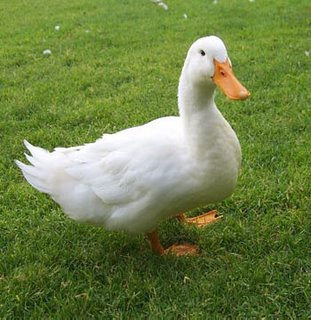
\includegraphics[width=7cm]{pato}
\label{pato}
\end{figure}

\begin{figure}[h]
\center
\caption{Mascote Tux}

\includegraphics[width=7cm]{tux}
\label{tux}
\end{figure}

\begin{figure}[h]
\center
\caption{Unicórnio Utópico}

\includegraphics[width=7cm]{unicorn}
\label{unicornio}
\end{figure}

A Equação \ref{pitagoras} é utilizada pelo Pato da Figura \ref{pato} para calcular suas hipotenusas.
\begin{equation}
a = \sqrt{b^2 + c^2}
\label{pitagoras}
\end{equation}


\end{document}